%%%%%%%%%%%%%%%%%%%%%%%%%%%%%%%%%%%%%%%%%%%%%%%%%%%%%%%%%%%%%%%%%
\chapter{INTRODUCTION TO DEEP LEARNING}
\label{ch:CH3}
%%%%%%%%%%%%%%%%%%%%%%%%%%%%%%%%%%%%%%%%%%%%%%%%%%%%%%%%%%%%%%%%%

In this section, first of all, we provide information on the basics of deep learning algorithms, and then we mention the loss function, and the optimization methods used to train deep learning algorithms. We conclude the section with the basics of convolutional neural networks (CNNs), CNN architectures used in this thesis, and the transfer learning concept.

\section{The Basics of Deep Learning}

Here we list basic terminologies associated with deep learning algorithms.

\begin{figure}[h]
	\centering
	% 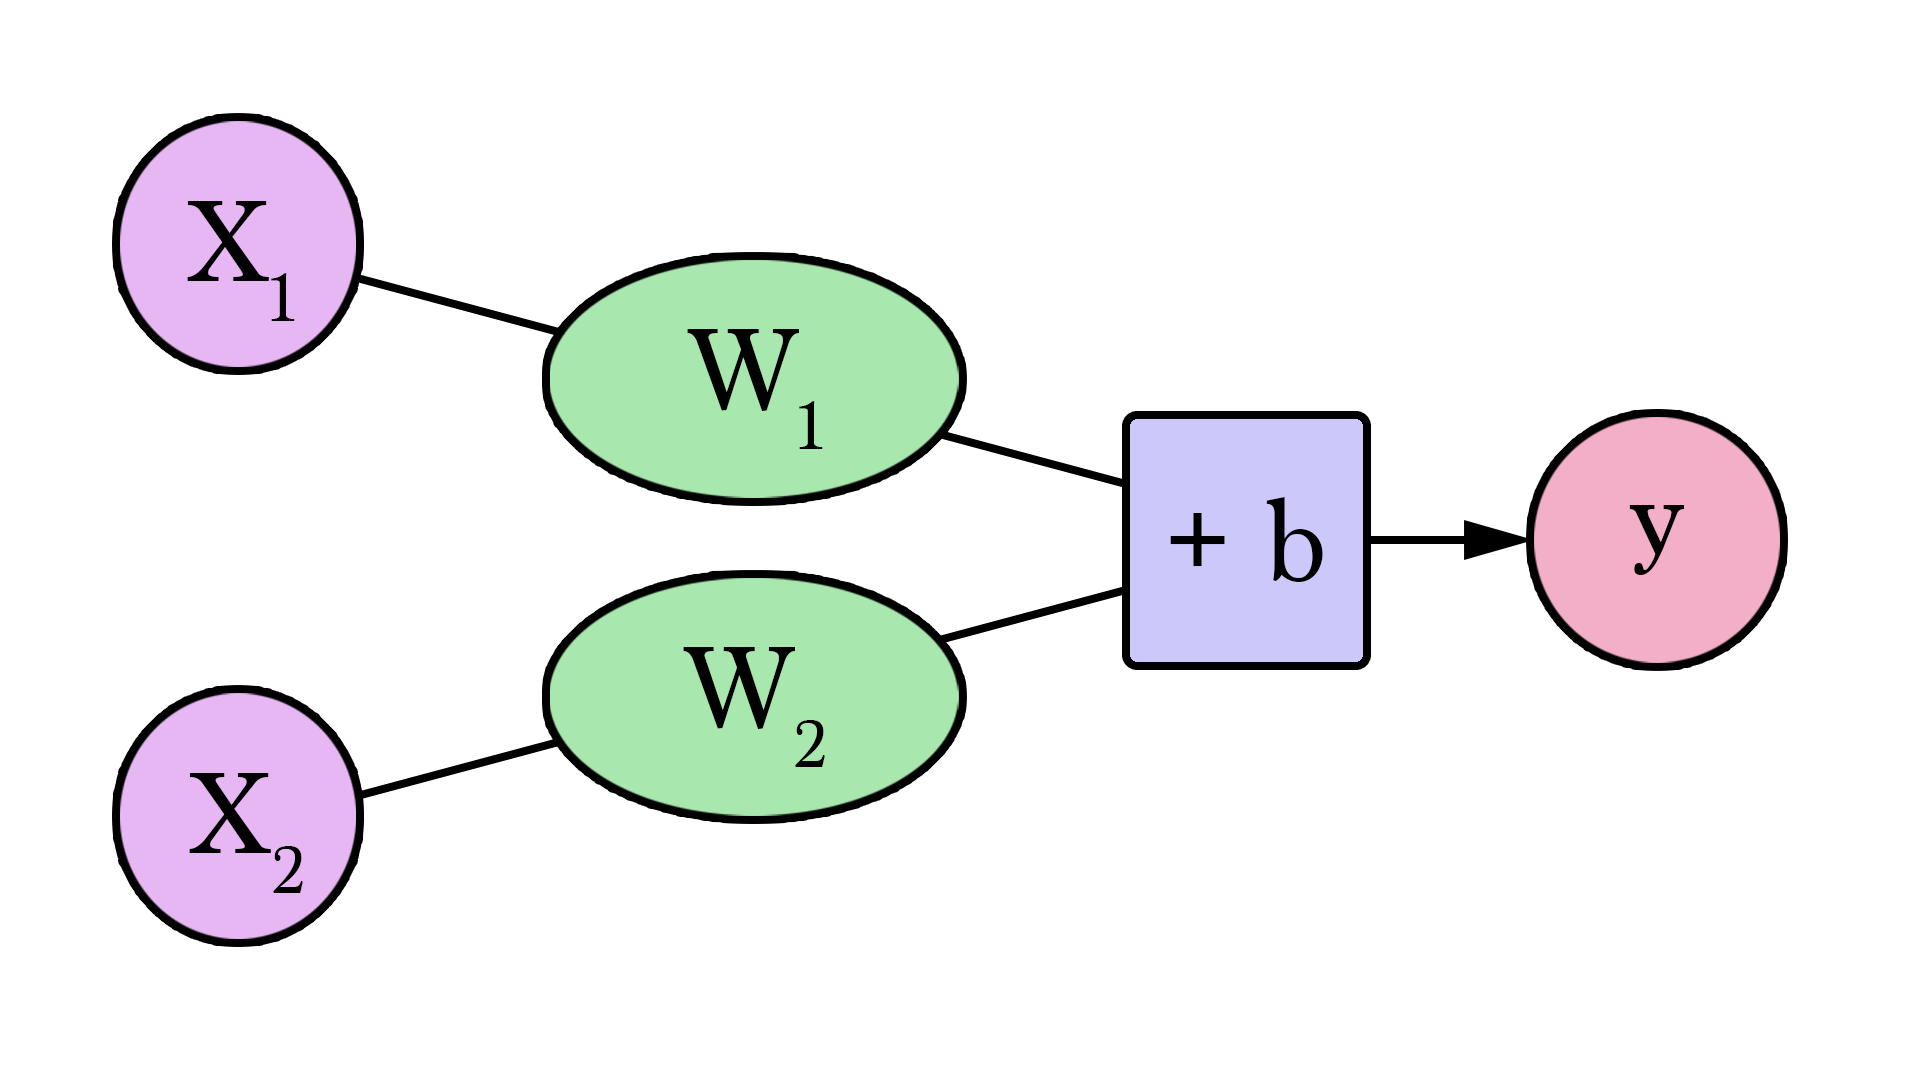
\includegraphics[width=.8\linewidth]{fig/NNs_2_variables.png}
	%\captionfootnotemark{A simple neural network with two neurons.}
	
	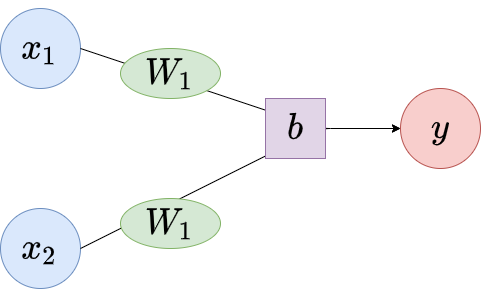
\includegraphics[width=.8\linewidth]{fig/simpleNN_2Neurons.png}
	\caption{A simple neural network with two neurons.}
	
	\label{fig:basic_neuron}
\end{figure}
% \footnotetext{Retrieved from GitHub: \hyperrefurl{https://jalammar.github.io/visual-interactive-guide-basics-neural-networks/} on March 28, 2021.}

\begin{itemize}
	
	\item \textbf{Neural Network}: A neural network is a learning framework for machines using a collection of functions over hidden layers to understand and translate an input data into a desired output. For a given input data, after the input layer reads the data, the hidden layers extract and transform the information and feed the output layer with them. The output layer is the final layer and it is used to obtain the outputs of one iteration of network in desired format. The main inspiration of neural networks is the human brain structure. A simple example for a neural network consisting of two neurons can be seen in Figure~\ref{fig:basic_neuron}, and the formulation for the output in this neural network is:
	
	\be 
	y = \textbf{W}^{T} \textbf{x} + b \:,
	\ee
	
	where $\textbf{x} \in \setsymbol{R}^{2}$ is the input vector, $\textbf{W} \in \setsymbol{R}^{2}$ is the weight vector, $b \in \setsymbol{R}$ is the bias term, and $y \in \setsymbol{R}$ is the scalar output.
	
	\item \textbf{Nodes (Neurons) and Links}:  Neural networks are made of nodes (neurons). The connections between the layer nodes are called as links. Each link has weight and bias parameters which are carried over neurons. Nodes receives the parameters of incident links, process them, and produces an output.
	
	\item \textbf{Weight and Bias}: Weight and bias terms are learnable parameters related to input data and they must be updated iteratively to reach the optimal cost value. At the initial iteration, they can be taken as zeros or a random initialization can be used. Both of them are transformed from input nodes to output nodes over the nodes of hidden layers via links in a neural network. Some sources include the bias term into the weight, and only use the weight value as well.
	
	\item \textbf{Feed-forward and Back-propagation}: Basically, a neural network which has no loops or cyclic links over nodes considered as a group of feed-forward networks. The direction of information flow is straight-forward. Input layer handles the input data, and the outputs of input layer goes through the hidden layer as input. There may be one or several number of hidden layers, and the output of each is the input of the next hidden layer. Finally, the output of last hidden layer feeds the output layer, and the output nodes forward their outputs to the loss function. During this process, the weights and bias values do not change. To update and find the most appropriate weight and bias values, back-propagation is used. To reach the optimal loss value, at each iteration of training, the negative gradient of the loss function is used to update the weight and bias terms. At the first iteration, this gradients are considered as zero or a random initialization is used. More information and examples can be found in Section~\ref{sec:basics_of_cnn}.
	
	\item \textbf{Epoch}: An epoch is an iteration when the train data passes forward and backward through the whole neural network only once. Generally, the train data passes through the whole network multiple times to optimize the learning process.
	
	\item \textbf{Batch}: If an epoch is too large to enter the neural network at once, data in the epoch can be dived into several smaller batches. Then, a batch is defined as a group of data samples selected from this data. The number of data samples in a batch are mostly chosen as a power of $2$ such as $2^4$, $2^5$, and  $2^6$ etc. If the train data enters the neural network in batches, then it is recommended to shuffle data order in each epoch before creating new batches from train data.
	
	\item \textbf{Train Data and Training}: The data group reserved to be used in learning process is called as train data. The ratio of train data size to whole data is generally determined as 7:10 or 8:10, and the rest of data is placed into the test data group. The train data must be strictly separated from validation and test data, and should be used on training process only. Training process consists of multiple epochs. At each epoch, the train data goes into the model as input, the neural network works for learning data, the losses and accuracy (if desired) are computed, and the losses are optimized. If batching is used, this process is applied onto each batch, and the average and final losses and accuracy (if desired) are calculated over all batches at the end of each epoch.
	
	\item \textbf{Validation Data and Validating}: If there exists enough train data for the problem and learning process, one may need validation data to validate the learning process periodically. The validation data group is strictly separated from train data such that its size is generally 70\% or 80\% of train data. During the validation process no optimization process is applied. For that reason, the weights and biases are stable. The losses and other desired metrics such as accuracy are computed only.
	
	\item \textbf{Test Data and Testing}: The data group reserved to be used in testing process is called as test data. The ratio of the size of test data to the whole data is generally determined as 2:10 or 3:10. The test data must be strictly separated from train data, and should be used on testing process only. The training process should not see any of test data. Testing process is usually applied at the end of all epochs. However, when the train data is not feasible to be divided into validation data, at the end of each epoch testing process may be applied on test data. This method is also used to determine the over-fitting and stop point.
	
	\item \textbf{Under-fitting and Over-fitting}: A learning algorithm may have under-fitting problem when it cannot capture or fit the data well. Under-fitting problem results in insufficient metrics during the training process since the learnable parameters are not optimized enough to reach at a satisfactory loss value. On the other hand, when the model fits the train data perfectly, it might have started to memorize the train data and may not learn something new from the data. Therefore, even though training metrics are nearly perfect, the testing metrics in the opposite direction of what is desired can be seen. The main reason for this is that the learnable parameters were directly adjusted for train data and not feasible for test data anymore. This situation is called as over-fitting. A validation set can be used to control the over-fitting by periodically checking the metrics of a data out of train set, while trying to rise above the under-fitting. By that way, a well-fitting or appropriate-fitting may be caught. The illustrations for three situations can be seen in the Figure~\ref{fig:underfitting_overfitting}.
	
	\begin{figure}[h]
		\centering
		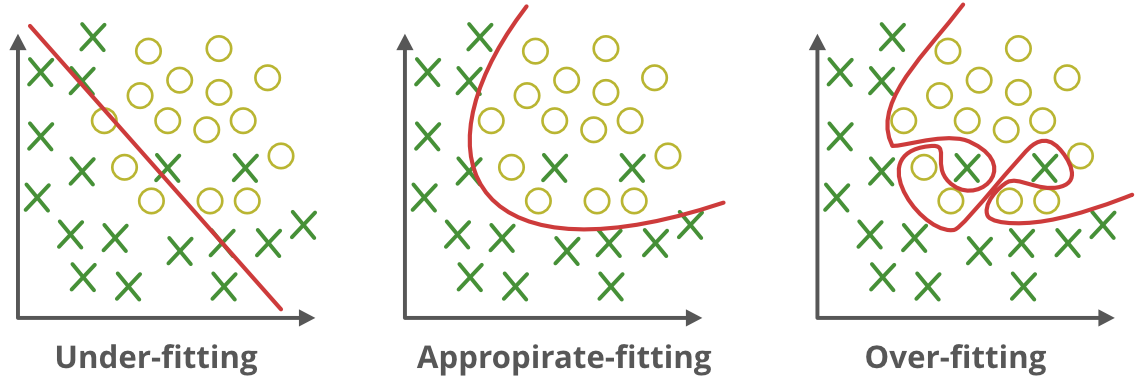
\includegraphics[width=1\linewidth]{fig/underfitting_overfitting.png}
		\vspace*{1mm}
		\captionfootnotemark{Illustration of under-fitting, well-fitting, and over-fitting of models to the data.}
		\label{fig:underfitting_overfitting}
	\end{figure}
	\footnotetext{Retrieved from GeeksforGeeks: \hyperrefurl{https://www.geeksforgeeks.org/underfitting-and-overfitting-in-machine-learning/} on March 28, 2021.}
	
\end{itemize}

\section{The Cross-Entropy Loss Function}\label{sec:CH3_cross_entropy}

Loss function is the function that represents the error between true and predicted values which can be called as the cost of the problem to be optimized.

The cross-entropy loss function is one of the most commonly used loss functions to measure the performance of a classifier. The cross-entropy function calculates the cost through the negative log-likelihood function \cite{negative-ll} which uses log class probability values computed by log-Softmax function \cite{logsoftmax}. Here the loss value increases together with the divergence between the grand-truth label and how likely this label is estimated.

The cross-entropy loss function for a sample, f, as a function of weights, is defined as given below:

\begin{equation}
	\label{eq:cross_entropy_loss_formulae}
	f(\theta) = - \sum_{i=1}^{n} y_{i} \log(p_{i}) \:,
\end{equation}

where $n$ is the total number of classes, $y_{i}$ is the observed class label, and $p_{i}$ is the estimated class probability, which is a function of weight, $\theta$, from the model of interest for the $i^{th}$ class, respectively, with restriction $\sum_{i=1}^{n}p_{i}=1$. Thus, for a binary classification problem, the cross-entropy loss function can be re-stated as:

\begin{equation}
	\label{eq:binary_cross_entropy_loss_formulae}
	f(\theta) = - \left ( y\:\log(p) + (1 - y)\:\log(1-p) \right ) \:,
\end{equation}

where $y$ is the binary variable with two class labels $1$ and $0$, where $1$, true class label, shows the presence of of the condition of interest, whereas $0$ shows the opposite, and and $p$ is the estimated probability for the true class label.

\section{The Basics of Optimization Methods}
\label{sec:CH3_the_basics_of_optimization}

Various optimization methods can be used for reducing the losses and reaching more accurate predictions. The weights are initialized and updated at each training epoch. The initialization strategies may vary depending on the neural network architecture. However, it is always aimed to achieve the most satisfying results by using some optimization algorithms called as optimizers.

\subsection{Stochastic Gradient Descent with Momentum  Optimization Algorithm}

Stochastic gradient descent (SGD) can be considered as a stochastic approximation of gradient descent optimization \cite{gradient_descent_algorithms} and is an iterative method for optimizing an objective function with suitable smoothness properties. The momentum remembers the weight update at each iteration and determines the next update as a linear combination of the gradient and the previous update \cite{SGD_Momentum}. An example for a pseudo-code for SGD with momentum optimization is given in Figure~\ref{fig:sgd_momentum}. Note that the weight parameter $\theta$ is denoted by $\textbf{x}$ in this figure.

\begin{figure}[h]
	\centering
	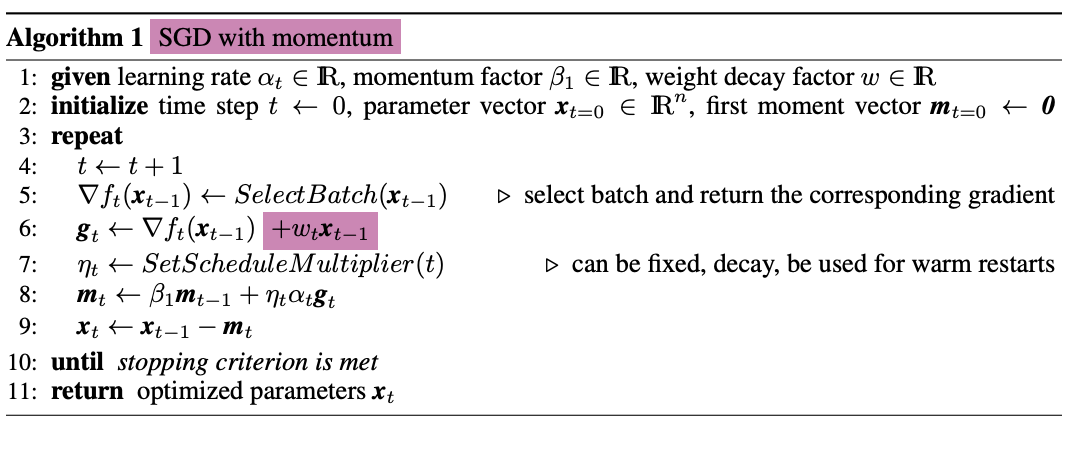
\includegraphics[width=\linewidth]{fig/sgd_momentum.png}
	\caption{A pseudo-code for SGD with momentum optimization \cite{weight_decay_regularization}.}
	\label{fig:sgd_momentum}
\end{figure}

\subsection{Adaptive Moment Estimation Optimization Algorithm}

Adaptive moment estimation (Adam) is an optimization algorithm that uses the running averages of both the gradients and the second moments of the gradients. Before each step, the gradient of loss function is calculated and a step in the opposite direction is taken with corresponding rate. This process is also called as Adam with L2 regularization \cite{Adam}. An example for a pseudo-code for Adam optimization is given in Figure~\ref{fig:adam_and_adamw}. Note that the weight parameter $\theta$ is denoted by $\textbf{x}$ in this Figure.

\subsection{Adam Decoupled Weight Decay Optimization Algorithm}

Adam decoupled weight decay optimization algorithm (AdamW) does not use the regularization as the normalized by square root of second moment vector. Thus, it is only proportional to the weight itself \cite{Adam}. An example for a pseudo-code for AdamW optimization is given in Figure~\ref{fig:adam_and_adamw}. Again, note that the weight parameter $\theta$ is denoted by $\textbf{x}$ in this figure.

The main difference of Adam and AdamW, as illustrated in Figure~\ref{fig:adam_and_adamw}, is that, the weight decay is directly applied to the gradient of loss function on Adam, while it is decoupled on AdamW. Hence, the weight decay affects moment vectors and appears both in numerator and denominator during weight parameter update. Furthermore, since it is in multiplicative form with learning rate parameter, the fine-tuning of learning rate and weight decay values become dependent to each other. On the other hand, weight decay is only applied at weight parameter update step, and it takes a separated charge during this update on AdamW.

\begin{figure}[h]
	\centering
	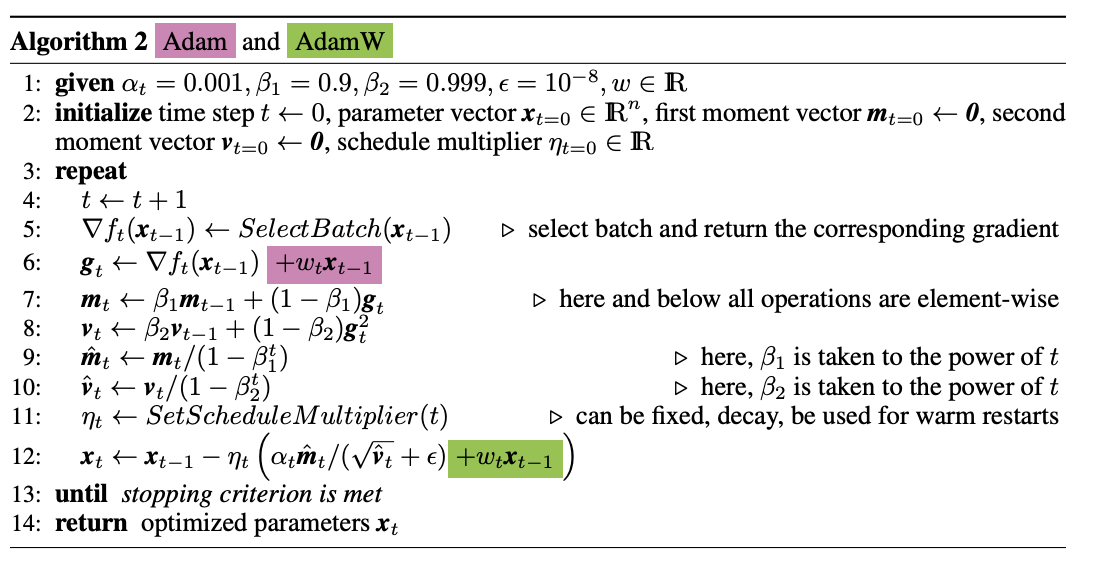
\includegraphics[width=\linewidth]{fig/adam_n_adamw.png}
	\vspace*{1mm}
	\caption{Pseudo-codes for Adam and AdamW optimization algorithms \cite{weight_decay_regularization}.}
	\label{fig:adam_and_adamw}
\end{figure}

\section{The Basics of Convolutional Neural Networks} 
\label{sec:basics_of_cnn}

The convolutional neural networks (CNNs) are the special research area of deep neural networks which are mostly used in analysis of visual problems. In this section, we give information on the fundamental layers and elements of CNN architectures. 

A CNN model basically consists of three main layers: 1) An input layer, 2) hidden layers, and 3) an output layer. For example, Figure~\ref{fig:basic_cnn_sample} is an example for a CNN model with six layers consisting of one input layer, four hidden layers, and one output layer.


\begin{figure}[h]
	\centering
	% 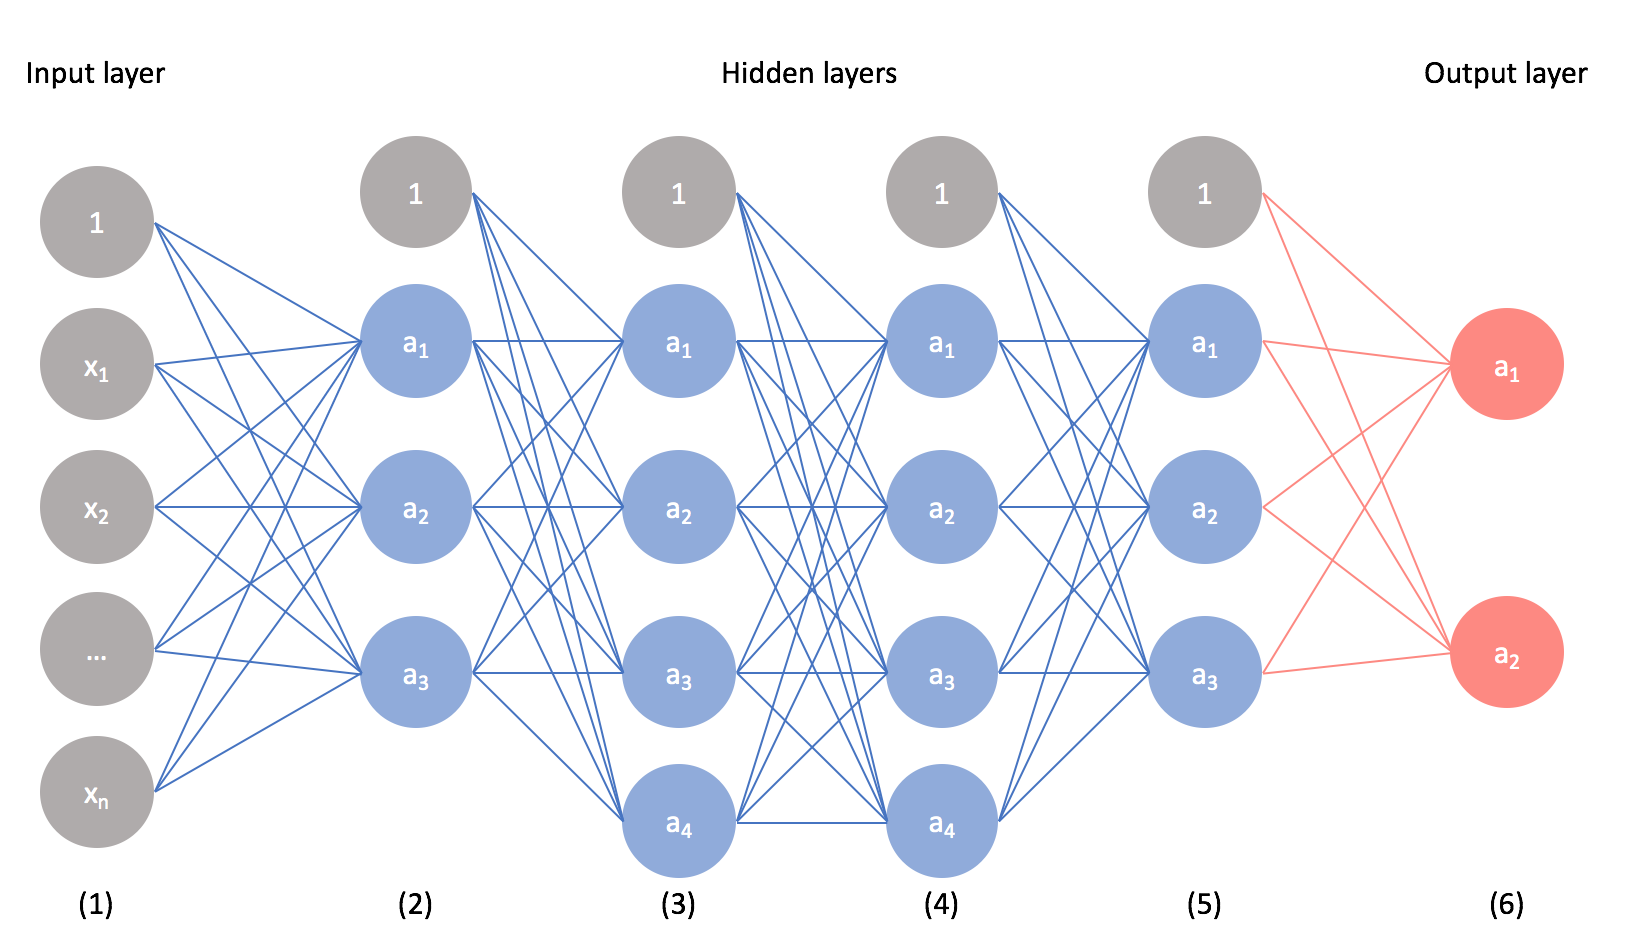
\includegraphics[width=14.5cm,height=14.5cm,keepaspectratio]{fig/basic_cnn_sample.png}
	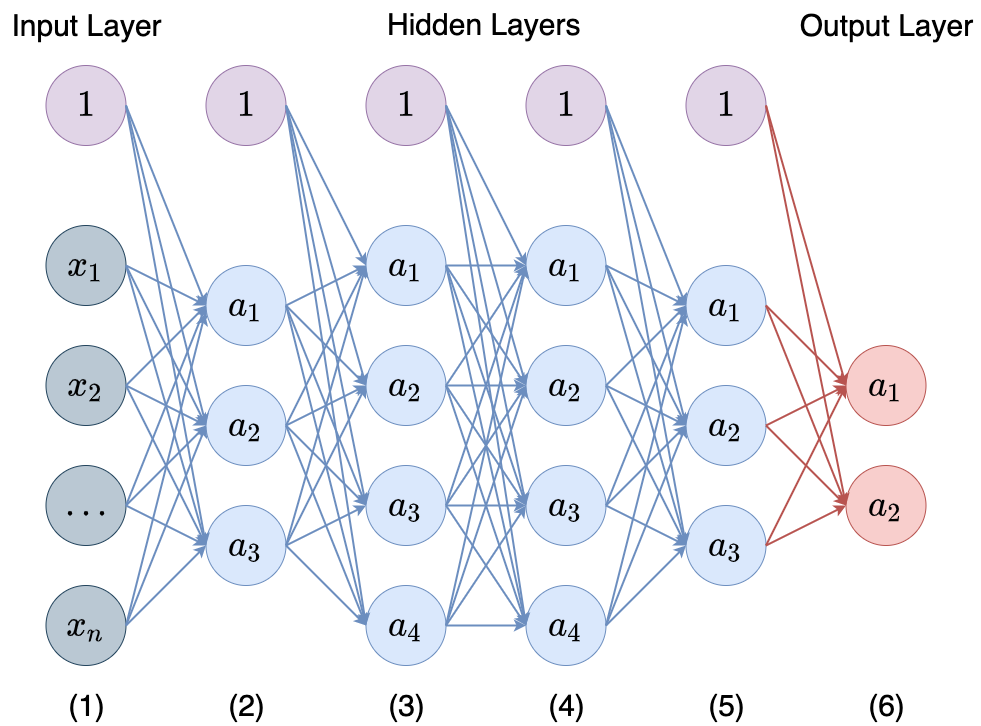
\includegraphics[width=13.5cm,height=13.5cm,keepaspectratio]{fig/simpleCNNarch.png}
	\vspace*{3mm}
	% \captionfootnotemark{An example for a simple CNN architecture.}
	\caption{An example for a simple CNN architecture.}
	\label{fig:basic_cnn_sample}
\end{figure}
% \footnotetext{Retrieved from: \hyperrefurl{https://www.jeremyjordan.me/convolutional-neural-networks/} on March 31, 2021.}


The structure of CNNs comports with the structure of feed-forward networks where the information goes through network in forward direction only. Back-propagation algorithm is commonly used to feed and train a feed-forward network. The algorithm orders to compute the gradients in weight space of a feed-forward network with respect to the loss function f(\textbf{$\theta$}). The weight matrix is defined as $\textbf{W} =(\theta_{1}^{T}, \dots ,\theta_{n^{(i)}}^{T}) \in \setsymbol{R}^{n^{(i)}} \times m^{(i)}$ where $n^{(i)}$ and $m^{(i)}$ are the number of inputs for $i^{th}$ layer and the size of each input in this layer, respectively. Then the weight space is updated with these gradients by the chosen optimizer such as SGD momentum, Adam, or AdamW. The gradient of objective loss function $f(\textbf{$\theta$})$ at a fixed weight vector \textbf{$\theta_{t}$} is computed via directional derivatives and chain rule and represented by $\nabla f(\textbf{$\theta_{t}$})$.

Let's consider a simple CNN architecture illustrated in Figure~\ref{fig:basic_cnn_sample} where each layer is denoted by    
$\textbf{a}^{(i)}$ with $i=1,2, \ldots, 6$. Assume there exists $n$ number of $x_{i}$ initial input nodes, where $\textbf{x} = \textbf{a}^{(1)} = (x_{1}, \dots , x_{n})$ is an n-dimensional input layer vector. 
Furthermore, the layers $\textbf{a}^{(i)}$, with $i=2, \ldots, 5$, are the hidden layers. For instance, $\textbf{a}^{(3)} = (a_{1}^{(3)}, a_{2}^{(3)}, a_{3}^{(3)}, a_{4}^{(3)})$ and $\textbf{a}^{(5)} = (a_{1}^{(5)}, a_{2}^{(5)}, a_{3}^{(5)})$. Lastly, the output layer feeding the loss function is $\textbf{a}^{(6)} = (a_{1}^{(6)}, a_{2}^{(6)})$, and the output $y$ value is determined by computing the class probabilities from $\textbf{a}^{(6)}$.

Then the gradient of loss function $f$ at the fixed weight vector $\theta_{t}$ is evaluated as:

\begin{equation}
	\nabla f (\theta_{t}) = 
	\begin{bmatrix}
		\frac { \partial f (\theta_{t})} {\partial \theta_{1}}\\
		\vdots \\
		\frac { \partial f (\theta_{t})} {\partial \theta_{n}}
	\end{bmatrix}.    
\end{equation} 

\begin{comment}
\textcolor{red}{Then, using directional derivatives and chain rule can be illustrated in Figure~\ref{fig:compute_gradient}.
Bu figuru sen mi cizdin? a1, a61, a2 de a6,2 olmali sanirim yukaridaki paragrafa bakarsak. bir de denklemi, denklem olarak ifade edersen, figur yerine iyi olur gibime geldi. i=1,2,..,n. n kullandım cunku CNN mimarsini gosteren figurde x katmani 1,..n. bir de figurde y bold ama denklemde bold degil.hangisi daha dogru acaba?}

\begin{figure}[h]
\centering
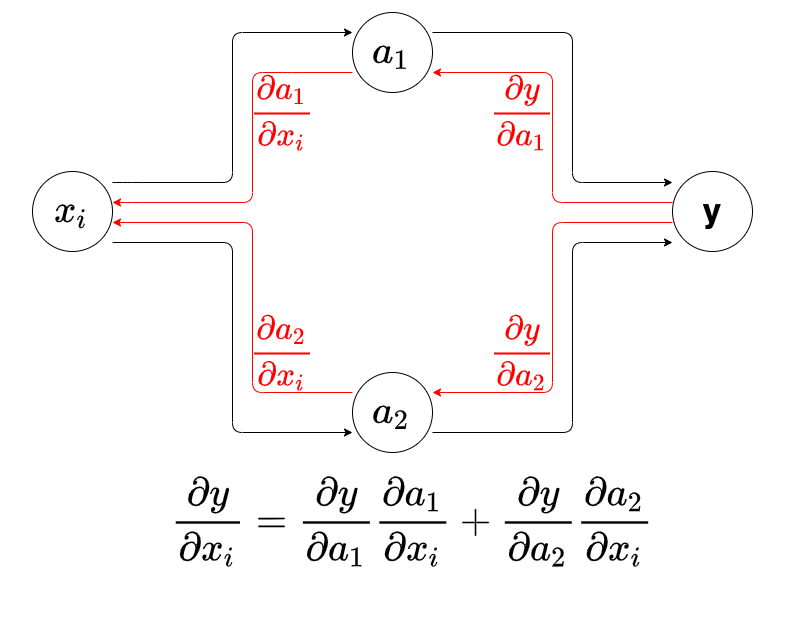
\includegraphics[width=.6\linewidth]{fig/gradient_example.png}
\vspace*{1mm}
\caption{An example for usage of directional derivatives and chain rule.}
\label{fig:compute_gradient}
\end{figure}
\end{comment}

The gray nodes in CNN architecture given in Figure~\ref{fig:basic_cnn_sample} are bias terms. Assume that the objective loss function is the cross-entropy loss function $f$ and our hypothesis function is to create a CNN architecture in the form $h_{i}: \setsymbol{R}^{k^{(i)}} \rightarrow \setsymbol{R}^{t^{(i)}}$, where $k^{(i)}$ and $t^{(i)}$ vary according to the corresponding layer. Then define $\textbf{a}^{(i)} = h_{i}(\textbf{W}^{(i)} \textbf{a}^{(i-1)} + b^{(i)})$ for each $i^{th}$ layer, where $\textbf{W}^{(i)}$ represents the weights of links from $i^{th}$ to $(i+1)^{th}$ layers, and $b^{(i)}$ is the bias term accompanying to these weights. Moreover, let us denote the weight of the link between the $j^{th}$ node of $i^{th}$ layer and the $z^{th}$ node of $(i+1)^{th}$ layer as $\textbf{W}_{j,z}^{(i)}$. We obtain the backward pass of our loss function with respect to the first weight matrix and bias terms by chain rule, respectively, as follows:


%\be
\begin{equation}
	\label{eq:compute_dl/dW}
	\frac{\partial f}{\partial \textbf{W}^{(1)}} = \frac{\partial f}{\partial \textbf{a}^{(6)}}  \frac{\partial \textbf{a}^{(6)}}{\partial \textbf{a}^{(5)}}  \frac{\partial \textbf{a}^{(5)}}{\partial \textbf{a}^{(4)}}  \frac{\partial \textbf{a}^{(4)}}{\partial \textbf{a}^{(3)}}  \frac{\partial \textbf{a}^{(3)}}{\partial \textbf{a}^{(2)}}  \frac{\partial \textbf{a}^{(2)}}{\partial \textbf{W}
		^{(1)}}\:\text{, and}
\end{equation} 
%\ee



%\be
\begin{equation}
	\label{eq:compute_dl/db}
	\frac{\partial f}{\partial b^{(1)}} = \frac{\partial f}{\partial \textbf{a}^{(6)}}  \frac{\partial \textbf{a}^{(6)}}{\partial \textbf{a}^{(5)}}  \frac{\partial \textbf{a}^{(5)}}{\partial \textbf{a}^{(4)}}  \frac{\partial \textbf{a}^{(4)}}{\partial \textbf{a}^{(3)}}  \frac{\partial \textbf{a}^{(3)}}{\partial \textbf{a}^{(2)}}  \frac{\partial \textbf{a}^{(2)}}{\partial b^{(1)}}\:\text{.}
\end{equation} 
%\ee



%Here, each partial derivative is computed as shown in Figure~\ref{fig:compute_gradient}. 
For instance, if the forward pass connection between $\textbf{a}_{2}^{(4)}$ and $\textbf{a}_{1}^{(5)}$ is $W^{(4)}_{2,1}$, we use the directional derivative rule while computing $\frac{\partial f}{\partial \textbf{a}^{(6)}}$ for the backward pass gradient to update $W^{(4)}_{2,1}$ value as: 


%\be
\begin{equation}
	\label{eq:compute_specific_weight}
	\frac{\partial f}{\partial W^{(4)}_{2,1}} = \frac{\partial f}{\partial \textbf{a}^{(6)}} \frac{\partial \textbf{a}^{(6)}}{\partial \textbf{a}_{1}^{(5)}}  \frac{\partial \textbf{a}_{1}^{(5)}}{\partial W^{(4)}_{2,1}} = \Big ( \frac{\partial f}{\partial \textbf{a}_{1}^{(6)}}  \frac{\partial \textbf{a}_{1}^{(6)}}{\partial \textbf{a}_{1}^{(5)}} + \frac{\partial f}{\partial \textbf{a}_{2}^{(6)}} \frac{\partial \textbf{a}_{2}^{(6)}}{\partial \textbf{a}_{1}^{(5)}} \Big )  \frac{\partial \textbf{a}_{1}^{(5)}}{\partial W^{(4)}_{2,1}} \:\text{.}
\end{equation} 
%\ee


In the same way, the gradient for $b^{(5)}$ can be computed as: 


%\be
\begin{equation}
	\label{eq:compute_specific_bias}
	\frac{\partial f}{\partial b^{(5)}} = \frac{\partial f}{\partial \textbf{a}^{(6)}}  \frac{\partial \textbf{a}^{(6)}}{\partial b^{(5)}} = \frac{\partial f}{\partial \textbf{a}_{1}^{(6)}}  \frac{\partial \textbf{a}_{1}^{(6)}}{\partial b^{(5)}} + \frac{\partial f}{\partial \textbf{a}_{2}^{(6)}}  \frac{\partial \textbf{a}_{2}^{(6)}}{\partial b^{(5)}}\:\text{.}
\end{equation} 
%\ee



\subsection{Convolutional Layer}

Convolutional layer is the building block of CNN architectures and is used to reveal the distinctive features of input data. A convolution layer includes one or multiple windows named as filter (or kernel) that can be of different sizes such as $2 \times 2$, $3\times3$, and so on. The coefficients, which are included in filters, change at each iteration during the training of a CNN. This coefficients and their updates are used to detect the significant and learnable parts of the data.

Filtering is started to be applied from the upper left corner of the image and keeps moving towards the right. When there are no cells left to be scanned on the right, it continues from the lower cells as before. At each step, the filter and the corresponding area of input matrix are multiplied by element-wise. The step length of scanning process is called as stride. The default stride value is 1; however, different stride values may be used depending on the input data and CNN architecture. If the stride is set as $s$, then the kernel window move by jumping $s$ cells. 

Sometimes, an inconsistency between filter, stride, and input layer sizes can be seen while trying to use desired convolutional layer. In this situation, the edges of input matrix may be filled by zeros. These process is called as padding. If the padding value is set as $p$, the $p$ cells with zero values are added to the edges of input matrix. This method can be also used to pay attention to the edges and corners of original input matrix.

\begin{figure}[!h]
	\centering
	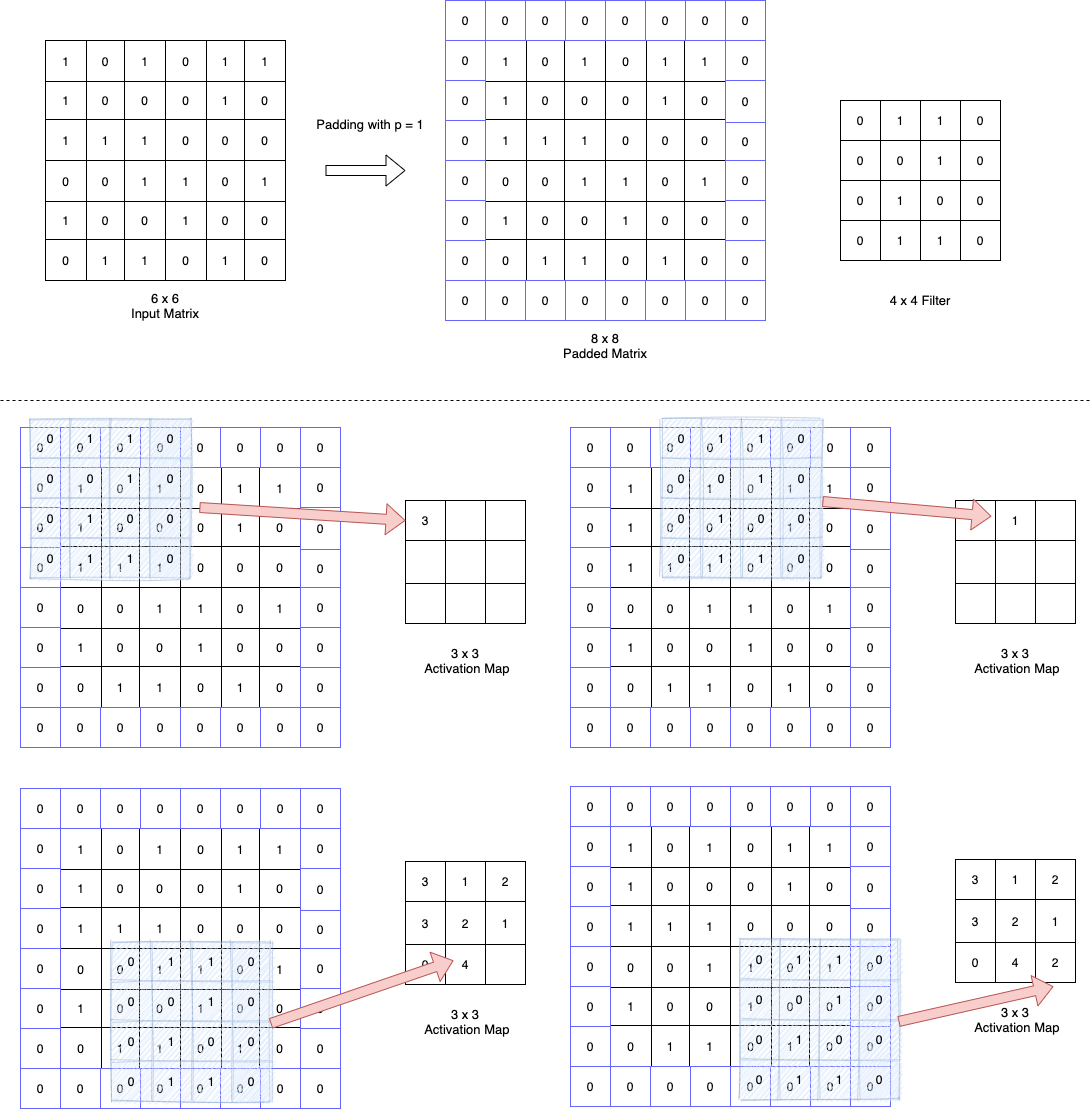
\includegraphics[width=\linewidth]{fig/conv_layer.png}
	\vspace*{2mm}
	\caption{Activation map construction with a filter window size of  $4 \times 4$ and stride value of $2$.}
	\label{conv_layer}
\end{figure}

The various filters can be applied onto the input data to reveal low and high-level feature maps. After convolution, the size of the input data changes depending on the filter (or kernel), stride, and padding choices. The outputs of the convolution layers are called activation maps.

The Figure~\ref{conv_layer} gives a summary about how activation map is constructed for a given input matrix and a filter.

Let us give another example to see the details about computations about it. Assume that the input data 
holds raw pixel values of an image of width $223$, height $223$, and three color channels red, green, and blue so that it has a size of $223 \times 223 \times 3$. Let's choose 2 filter windows in the size of $5 \times 5$, the stride (step size) as $2$, and the padding size as $1$. If we denote the input size by $W_{input} \times H_{input} \times D_{input}$, the padding by $P$, the number of filters by $K$, the size of a filter window by $F \times F$ and the stride by $S$, then we have: 

\begin{itemize}
	\item $W_{input} = 223, \: H_{input} = 223, \: D_{input} = 3$,
	\item $K = 2, \: F = 5$,
	\item $P = 1, \: \text{and} \: S = 2$.
\end{itemize}

The size of activation map is calculated as:

\begin{flalign}
	\label{activation_map_w_output}
	&W_{output} = ((W_{input} - F + 2P)\,/\,S) + 1\:, \\
	\label{activation_map_h_output}
	&H_{output} = ((H_{input} - F + 2P)\,/\,S )+ 1\:,\quad\text{and} \\
	\label{activation_map_d_output}
	&D_{output} = K\:.
\end{flalign}

Consequently, the activation map of size of $112 \times 112 \times 2$ is produced through the equations  (\ref{activation_map_w_output}), (\ref{activation_map_h_output}), and (\ref{activation_map_d_output}) respectively. 

\subsection{Rectified Activation Function}

The activation function forms the output of the node for a given input or input set. Rectifier activation function maps the input to non-negative values. A unit form of the rectifier activation function, which is given in equation (\ref{eq:relu_formula}), is called as Rectified Linear Units (ReLU) which is the most common used in neural networks. ReLU is defined as:

\begin{equation}
	\label{eq:relu_formula}
	f(x) = \max(0, x) \:.
\end{equation}

\subsection{Pooling Layer}

Pooling layers  are commonly used in between the convolutional layers, especially after activation functions. A pooling layer outputs a new feature map with the lower size than the size of input feature map.  The characteristics of output feature map depends on the type of pooling layer. The pooling layers have a stride parameter to control the step size of the movement of pooling window. The most common pooling functions are given below. Moreover, a simple example on maximum pooling can be found in Figure~\ref{fig:maxpooling}.

\begin{itemize}
	\item \textbf{Average Pooling:}  The average of corresponding window is computed and inserted into output feature map.
	\item \textbf{Maximum Pooling:}  The maximum value of corresponding window is inserted into output feature map.
\end{itemize}

\begin{figure}[h]
	\centering
	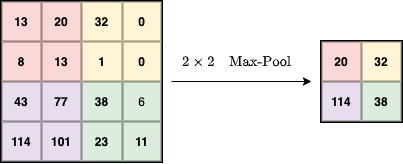
\includegraphics[width=1.0\linewidth]{fig/maxPool.png}
	\vspace*{1mm}
	\caption{Maximum pooling operation sample with 
		$2 \times 2$ window and stride value of 2.}
	% 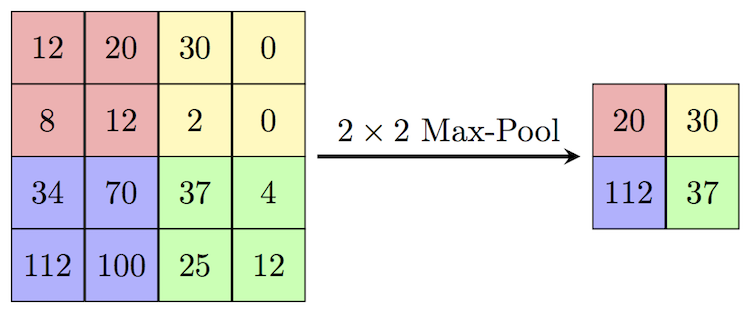
\includegraphics[width=.8\linewidth]{fig/MaxpoolSample.png}
	% \captionfootnotemark{Maximum pooling operation sample with 
	% $2 \times 2$ window and stride value of 2.}
	\label{fig:maxpooling}
\end{figure}
% \footnotetext{Retrieved from: \hyperrefurl{https://computersciencewiki.org/index.php/Max-pooling_/_Pooling} on April 3, 2021.}

\subsection{Batch Normalization}

Batch normalization is a technique for training the deep neural networks that standardize the inputs to one layer for each mini batch. This has the effect of stabilizing the learning process and significantly reducing the number of training epochs required \cite{A_novelCNNModel}.

\subsection{Drop-out}

Drop-out is the removing operation of the nodes below certain threshold value in the network at each training iteration. In other words, it is aimed not to use weak information and memorize the network. Drop-out can be in any layer and its threshold value, which can differ in different layers,  is between [0,1]. An illustration about drop-out can be seen in the Figure~\ref{fig:dropout}.

\begin{figure}[h]
	\centering
	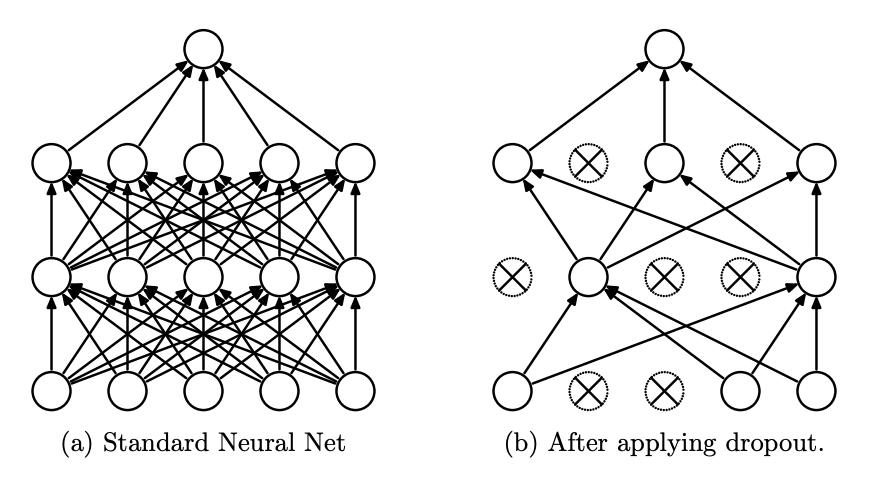
\includegraphics[width=.8\linewidth]{fig/dropout.png}
	\caption{(a) A standard neural network, (b) A neural network after applying drop-out\cite{dropout_article}.}
	\label{fig:dropout}
\end{figure}

\subsection{Flattening}

Flatten operation reshapes the input into the one-dimension. It is used before passing to the fully-connected layers.

\subsection{Fully-Connected Layer}

This structure is used to combine the information in the previous layers. It requires the flatten operation before itself. The fully-connected layers are used to classify data in different categories, or construct feature maps to be used in another artificial network methods.A simple fully-connected layer is given in the figure~\ref{fig:fully_connected_layer}.

\begin{figure}[h]
	\centering
	%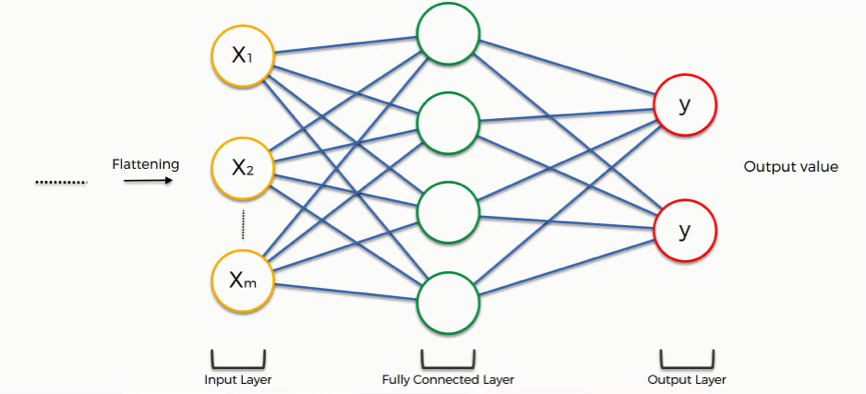
\includegraphics[width=\linewidth]{fig/fully_connected_layer.png}
	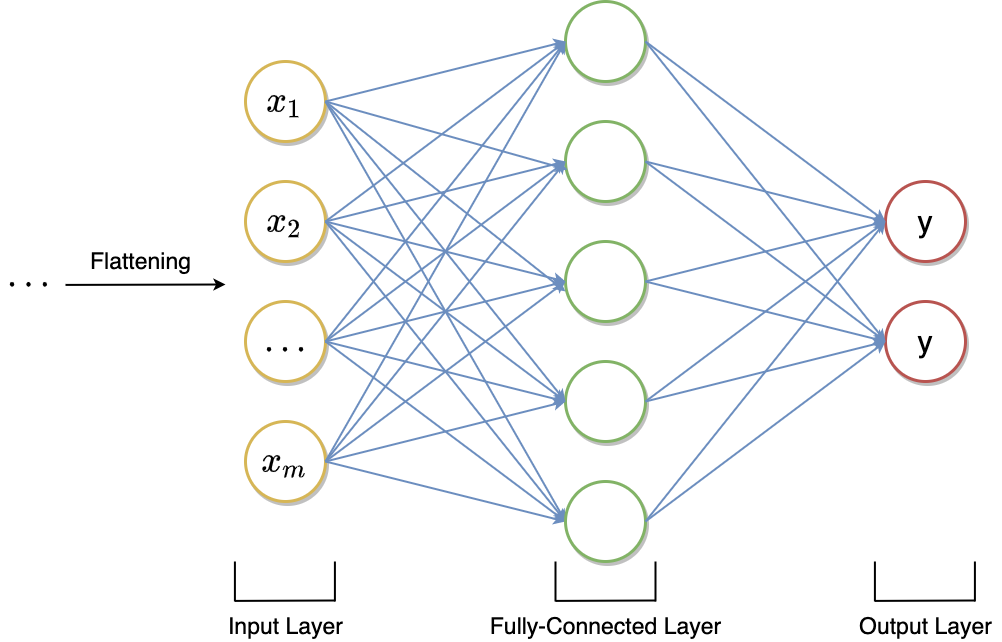
\includegraphics[width=.8\linewidth]{fig/fullyConnected.png}
	\vspace*{2mm}
	\caption{The usage of a full-connected layer for a binary classifier.}
	%\captionfootnotemark{The usage of a full-connected layer for a binary classifier.}
	\label{fig:fully_connected_layer}
\end{figure}
%\footnotetext{Retrieved from: \hyperrefurl{https://www.superdatascience.com/blogs/convolutional-neural-networks-cnn-step-4-full-connection} on April 3, 2021.}

\section{Transfer Learning} \label{CH3:transfer_learning}

Transfer learning is transferring the weights, features etc. in a pre-trained model to another artificial learning model. This can be between two different deep learning models or across a machine learning and a deep learning model. In this thesis, the weight transfer from pre-trained CNN models to CNN models and feature transfer from CNN models to machine learning models are used.

Transfer learning is generally used to shorten the training time if the data set is insufficient and to achieve high performance with less data. If the data on each class is less than 1000, the data set may be considered as small. 

To prepare a pre-trained CNN model for visual artificial intelligence problems, ILSVRC 2012 ImageNet \cite{imagenet} data set, including 1000 class with large data, is commonly used. The weights after the training process is saved and shared to use in transfer learning afterwards. In transfer learning, the pre-trained model is called with its pre-computed weights, and the weights are transferred into the same empty neural network. There exists different approaches to train this new neural network; such that, training the all layers on the convolutional block, training a part of the layers on the convolutional block and freezing the others, and freezing all layers on the convolutional block. The choice of strategy, which is called as fine-tuning operation, depends on the size of data set and the similarity between the data set used in pre-training process and the data set to be used in current task. Then the last fully-connected layer is adapted to the current task by updating itself or adding new fully-connected layers. The mentioned three strategies can be seen in the Figure~\ref{fig:pretrain_strategies}.

\begin{figure}[h]
	\centering
	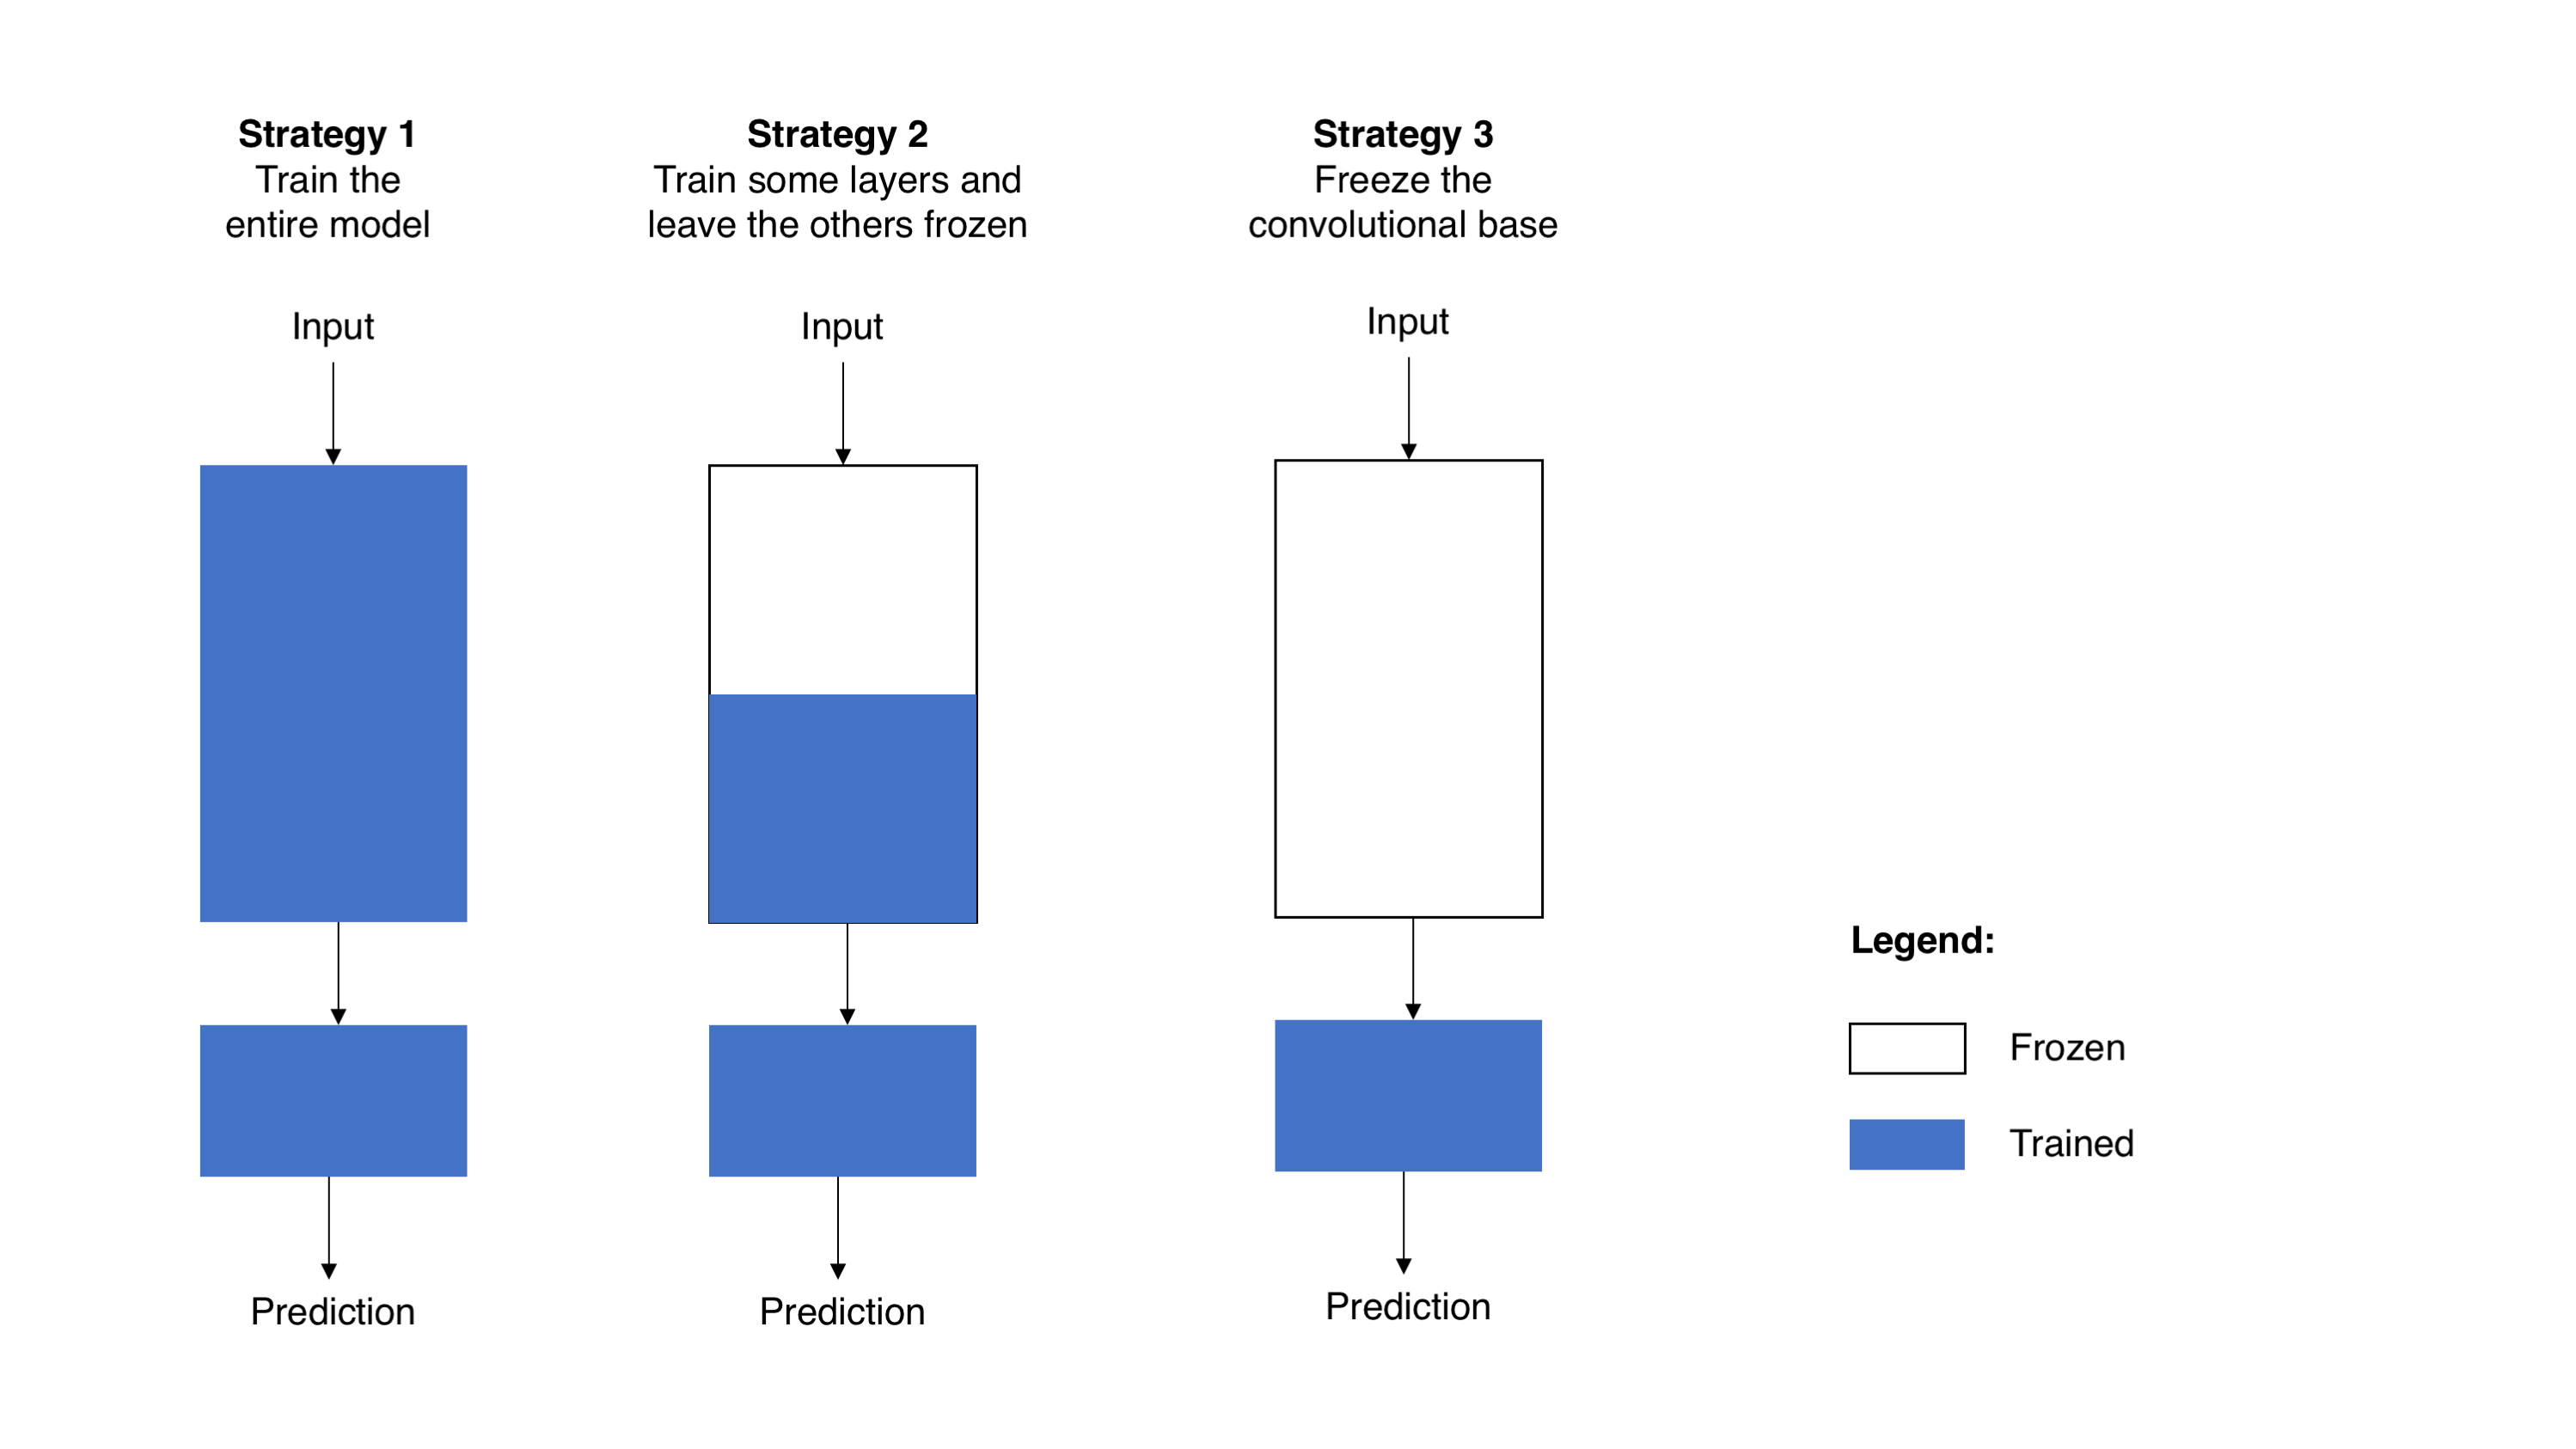
\includegraphics[width=.8\linewidth]{fig/pretrain_strategies.png}
	\vspace*{1mm}
	\captionfootnotemark{Different fine-tuning strategies on a pre-trained model.}
	\label{fig:pretrain_strategies}
\end{figure}
\footnotetext{Retrieved from: \hyperrefurl{https://towardsdatascience.com/transfer-learning-from-pre-trained-models-f2393f124751} on April 3, 2021.}

On the other hand, to prepare a deep feature set to be used in another artificial learning model, such as machine learning models, the features on a fully-connected layer, mostly the first or second, are extracted and saved. Then the saved deep features are used in the target artificial learning model as the feature map of data set. A real application of deep feature transfer learning as a road-map, which also used in this thesis, can be found in Figure~\ref{fig:A_novelCNNModel_architecture}.

\begin{figure}[h]
	\centering
	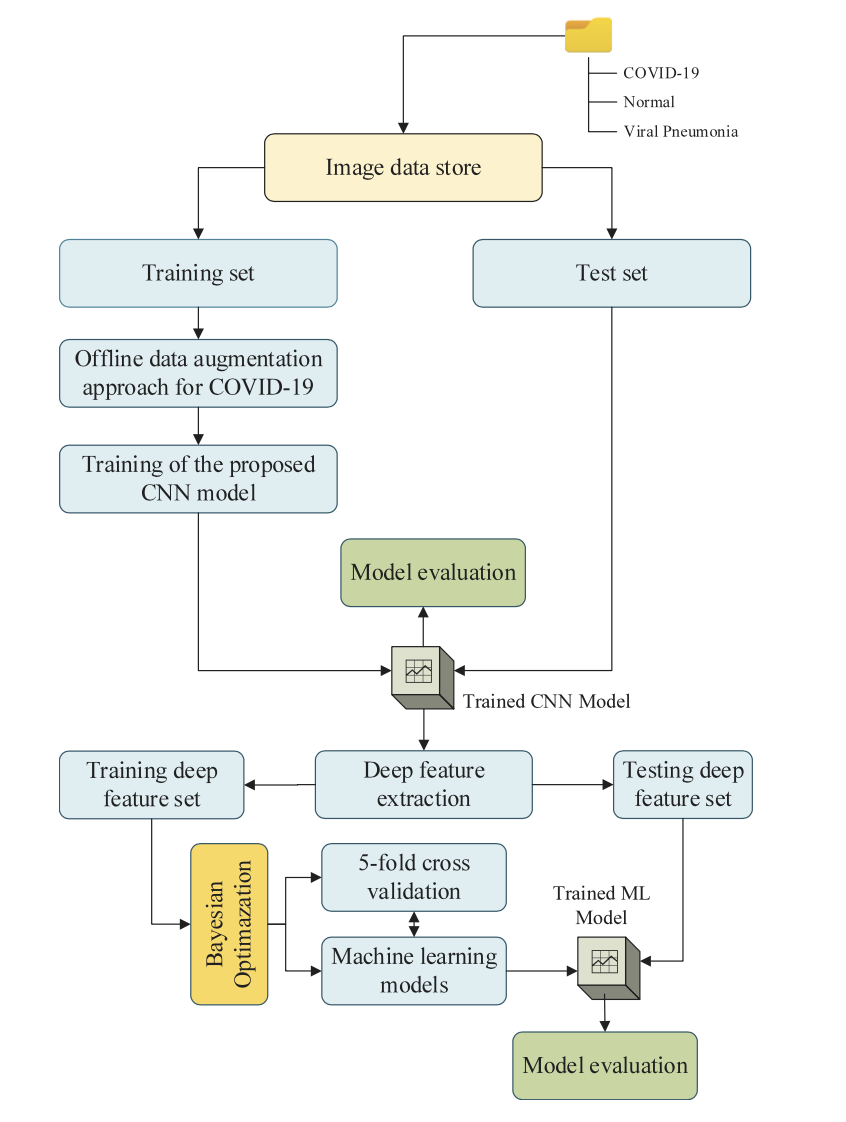
\includegraphics[width=.8\linewidth]{fig/deepfeauter_usage.png}
	\caption{Deep feature extraction from CNN models and using them in machine learning models \cite{A_novelCNNModel}.}
	\label{fig:A_novelCNNModel_architecture}
\end{figure}

\section{CNN Models}

There are several CNN architectures which can be simply called as models. These models consist of various combinations of input layer, hidden layers and an output layer such that some basics of them are explained in Section~\ref{sec:basics_of_cnn}.

In this section, the state-of-the-art CNN models used in this thesis are introduced and detailed.

\subsection{AlexNet}

The AlexNet architecture was developed by Krizhevsky et al. \cite{AlexNet} for the object recognition problem. This model was trained with the ILSVRC 2012 ImageNet \cite{imagenet} dataset, achieved high performance results, and won the first place in the ImageNet competition in 2012. There are $9$ layers in total in the AlexNet architecture. Following the input layer, there are five convolution layers which use filters of size of $11 \times 11$ with a stride value of $4$, where some layers are supported by the maximum pooling layers as shown in Figure~\ref{fig:alexnet_arch}. The remaining three layers are the fully-connected layers which have the sizes of $2048$, $2048$, and the number of classes, respectively. In Figure~\ref{fig:alexnet_arch}, the number of classes are considered as 1000; thus, the last fully-connected layer has the size of $1000$.  The ReLU activation function is used after each convolution and fully-connected layer. The number of filters used increases as going deeper into the model.

\begin{figure}[h]
	\centering
	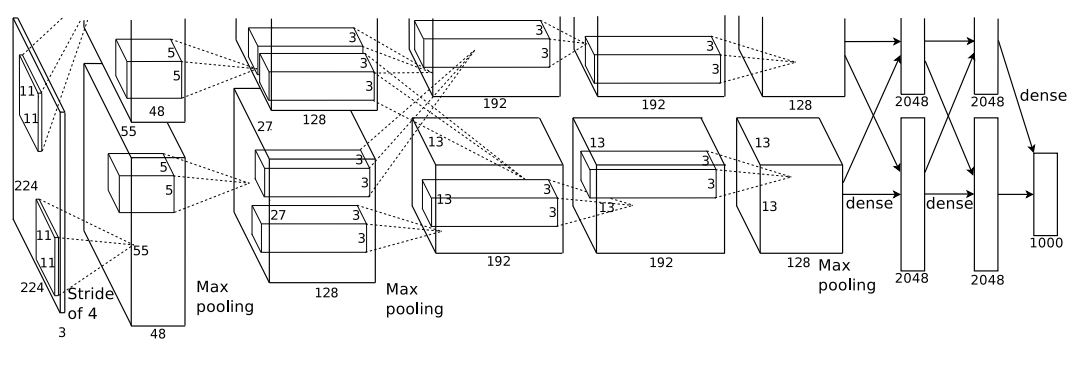
\includegraphics[width=\linewidth]{fig/alexnet_arch.png}
	\caption{Illustration of AlexNet architecture with a size of $224 \times 224 \times 3$ input image and 1000 class prediction support.\cite{AlexNet}.}
	\label{fig:alexnet_arch}
\end{figure}

\subsection{Residual Neural Networks}

The residual neural network (ResNet) architectures was proposed by He et al. \cite{ResNet} to avoid vanishing and exploding gradient problems by using residual blocks which is a simple connection which takes the activation from one layer and feeds it to another layer in much deeper. This model resulted in high performance results on ILSVRC 2015 ImageNet \cite{imagenet} data set and won the 1st place on the corresponding task. In the Figure~\ref{fig:residual_block}, it can be seen that the layer $a^{[l]}$ feeds two subsequent layers, namely, $a^{[l+1]}$ and $a^{[l+2]}$.

\begin{figure}[h]
	\centering
	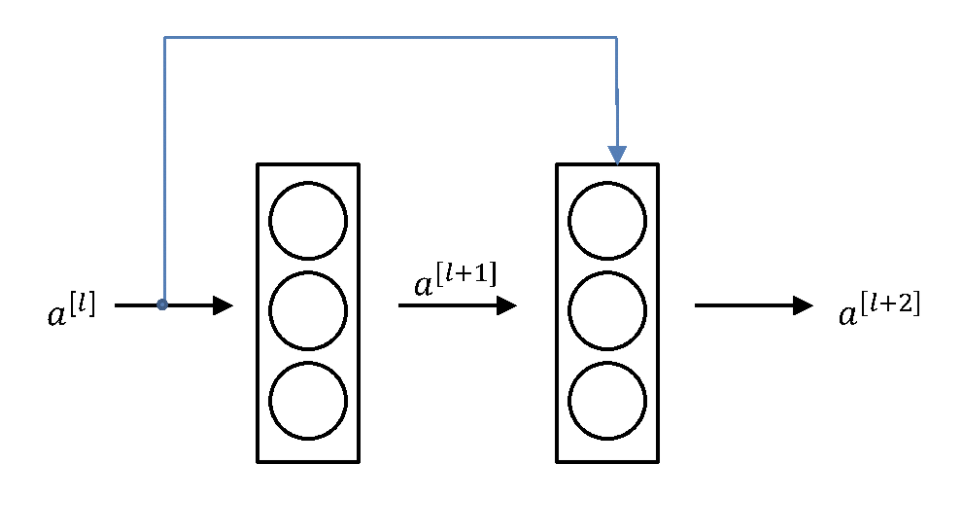
\includegraphics[width=.6\linewidth]{fig/residual_block.png}
	\captionfootnotemark{An illustration for residual block. Here, $a^{[l]}$ is the starting activation layer and $a^{[l+2]}$ is the fed activation layer.}
	\label{fig:residual_block}
\end{figure}
\footnotetext{Retrieved from: \hyperrefurl{http://datahacker.rs/deep-learning-residual-networks/} on April 4, 2021.}

Depending on the number of layers, there are a variety of special ResNet architectures which are briefly mentioned below.

\subsubsection*{\textit{ResNet-18}}

The first convolution layer includes a filter with a size of $7 \times 7$ and scans with a stride value of 2, then maximum pooling is applied with a $2 \times 2$ window along with a stride value of 2. Afterwards, 8 residual blocks, where each includes 2 convolutional layers with $3 \times 3$ filters, come. Hence, there exists 16 convolutional layers inside of residual blocks. After the residual blocks, there is an average pooling following a fully-connected layer with neurons in the size of the number of classes, which is 1000 in Figure~\ref{fig:resnet_archs}.

\subsubsection*{\textit{ResNet-34}}

The first convolution layer includes a $7 \times  7$ filter and scans with a stride value of 2, then maximum pooling is applied with $2 \times  2$ window and stride value of 2. Afterwards, 16 residual blocks, such that each of them includes 2 convolutional layers with $3 \times 3$ filters, come. That is, there exists 32 convolutional layers inside of residual blocks. After the residual blocks, there is an average pooling following a fully-connected layer with neurons in the size of the number of classes, which is 1000 in Figure~\ref{fig:resnet_archs}.

\subsubsection*{\textit{ResNet-50}}

The first convolution layer includes a $7 \times 7$ filter and scans with a stride value of 2, then maximum pooling is applied with  $2 \times 2 $ window and stride as 2. Afterwards, 16 residual blocks, such that each of them includes 3 convolutional layers with $1 \times 1$, $3 \times 3$ and $1 \times 1$ filters in order, come. That is, there exists 48 convolutional layers inside of residual blocks. After the residual blocks, there is an average pooling following a fully-connected layer with neurons in the size of the number of classes, which is 1000 in Figure~\ref{fig:resnet_archs}.

\begin{figure}[h]
	\centering
	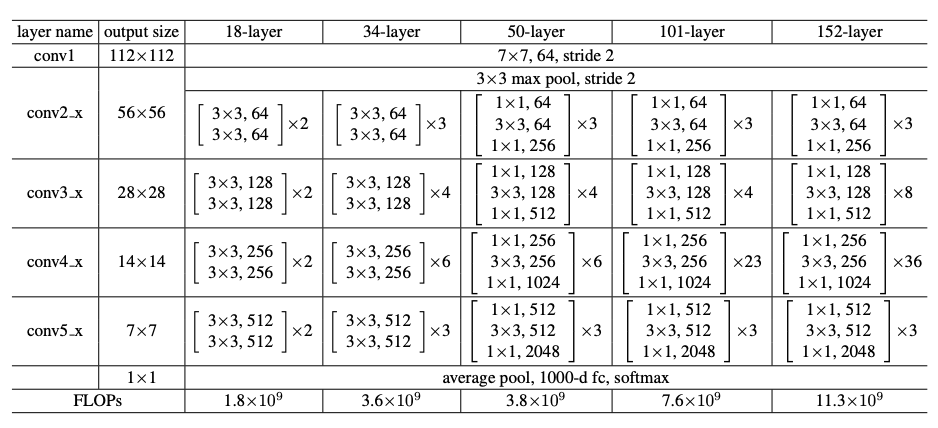
\includegraphics[width=\linewidth]{fig/resnet_archs.png}
	\vspace*{1mm}
	\caption{The architectures of ResNet-18, ResNet-34, and ResNet-50 \cite{ResNet}.}
	\label{fig:resnet_archs}
\end{figure}


\subsection{Visual Geometry Group}

Simonyan and Zisserman \cite{VGG} proposed a very profound architecture for the problem of image recognition. It is aimed to achieve higher classification performance by using a small size filter and increasing the depth of the model. This model was trained with the ILSVRC 2012  ImageNet \cite{imagenet} dataset and achieved high success results. This study has showed the importance of depth in image description models. The two types of Visual Geometry Group (VGG) architectures explained below can be seen in Figure~\ref{fig:vgg16_vgg19_archs}. In the figure, the number of classes are considered as 1000.

\begin{figure}[h]
	\centering
	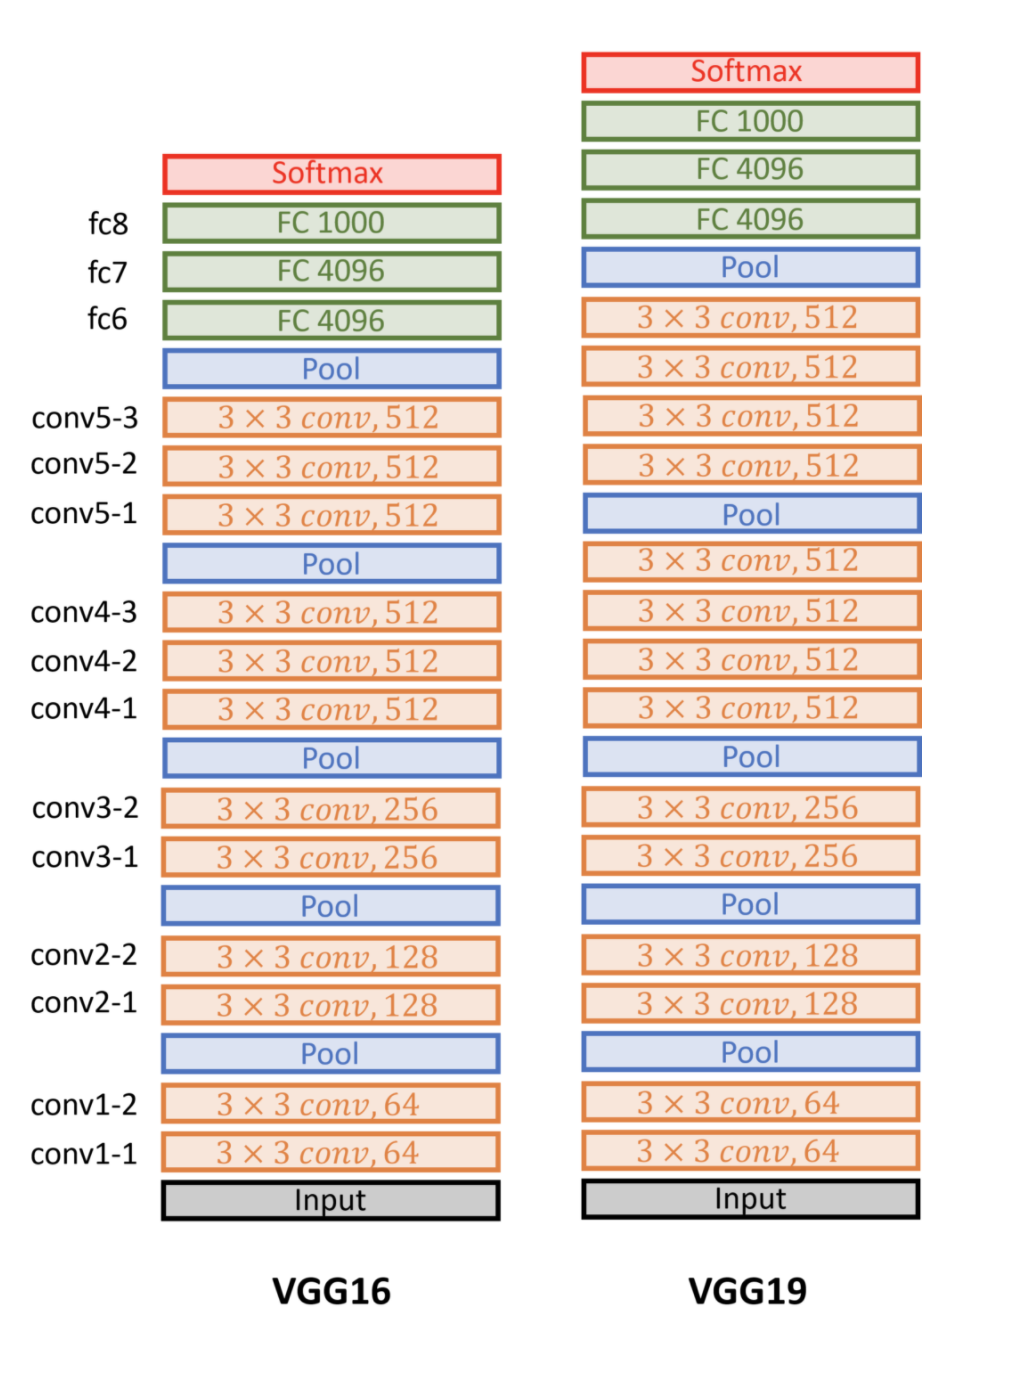
\includegraphics[width=.6\linewidth]{fig/vgg16_vgg19_archs.png}
	\captionfootnotemark{An illustration of VGG architectures.}
	\label{fig:vgg16_vgg19_archs}
\end{figure}
\footnotetext{Retrieved from: \hyperrefurl{http://datahacker.rs/deep-learning-vgg-16-vs-vgg-19/} on April 4, 2021.}

\newpage

\subsubsection*{\textit{VGG16}}

The model architecture starts with an input layer, and there are following 12 convolution layers using $3 \times 3$ filters. There are a total of 5 maximum pooling layers used after some convolution layers. In maximum pooling, $2 \times 2$ windows were used with stride as 2. After the convolution layers, there are three fully-connected layers such that the first two of which have 4096 neurons and the last one has neurons in the size of the number of classes, which is 1000 in Figure~\ref{fig:vgg16_vgg19_archs}. The ReLU activation function was used after all the hidden layers.

\subsubsection*{\textit{VGG19}}

The model architecture starts with an input layer, and there are following 14 convolution layers using $3 \times 3$ filters. There are a total of 5 maximum pooling layers used after some convolution layers. In maximum pooling, $2 \times 2$ windows were used with stride as 2. After the convolution layers, there are three fully-connected layers such that the first two of which have 4096 neurons and the last one has neurons in the size of the number of classes, which is 1000 in Figure~\ref{fig:vgg16_vgg19_archs}. The ReLU activation function was used after all the hidden layers.